%________________________________________________________________________________________________
\documentclass{beamer}
%________________________________________________________________________________________________
\usepackage[french]{babel} 
\usepackage[utf8]{inputenc} 
\usepackage[T1]{fontenc} 
\usepackage{graphicx}
\usepackage[utf8]{inputenc}
\usepackage{fancyhdr}
\usepackage{geometry}
\usepackage{tabularx,tabulary}
\usepackage{movie15}
%________________________________________________________________________________________________
\title{3I013 Réunion du 22 Mars 2019}
\author{Daoud KADOCH\\Fabien MANSON\\Maël FRANCESCHETTI\\Nicolas CASTANET\\}
%________________________________________________________________________________________________
%ce theme est le plus clean de Beamer le truc a ne pas utiliser c'est 'Warsaw'
\usetheme{default}
%suppression de la barre de navigation inutile
\setbeamertemplate{navigation symbols}{}
\setbeamertemplate{frametitle}[default][center]

%\logo{
\includegraphics[height=0.5cm]{logo_sorbonne.png}}

%________________________________________________________________________________________________
\addtobeamertemplate{footline}{
	\begin{flushright}
	\vbox{\insertframenumber/\inserttotalframenumber}
	\end{flushright}}

%________________________________________________________________________________________________
\begin{document}


	%premiere diapo
	\begin{frame}
		\begin{center}
		\date{21 mars 2019}
		\maketitle
		Ceci est la première diapo !\\
		\end{center}
	\end{frame}
	
	
	
	\begin{frame}
		\section{}
		\begin{flushleft}
		\frametitle{Sommaire}
		\tableofcontents{}
		\end{flushleft}
	\end{frame}
	
	
	\begin{frame}
	\section{Mavlink}
		\begin{center}
		\frametitle{Mavlink}
		%\subsection{Contraintes}
        %\framesubtitle{Les solutions}
        Deux solutions pour la création d'un fichier au format mavlink:
        
           	\begin{itemize}
                \item Création depuis le sdk C de Parrot
                \item Création depuis l'application de saisie de plan de vol map JavaScript
            \end{itemize}
            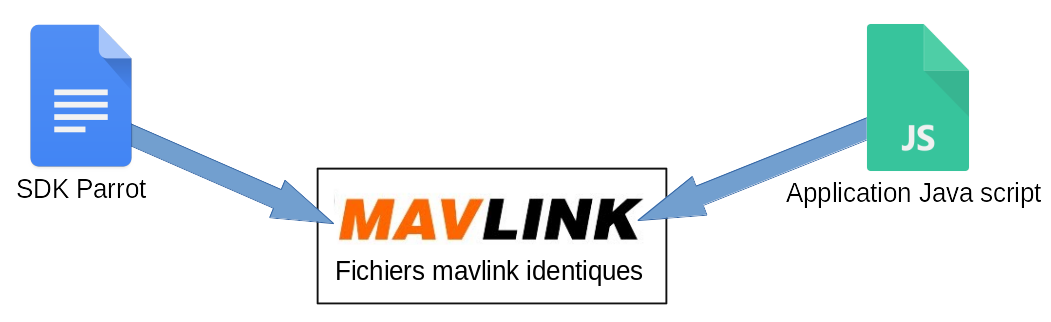
\includegraphics[scale=0.40]{schema_js_vs_sdk.png}
		\end{center}
	\end{frame}
	
	\begin{frame}
		\begin{center}
		\frametitle{Mavlink}
		%\subsection{Contraintes}
        %\framesubtitle{Les solutions}
           	\begin{itemize}
                \item Envoi du fichier mavlink au drone en ftp dans le code C
                \item Callbacks pour récupération des changements d'état de des erreurs pour les logs
                \item Envoi de la demande d'éxécution du mavlink au drone
            \end{itemize}
		\end{center}
	\end{frame}
	
	\begin{frame}
	\section{iPod et video en local}
		\begin{center}
		\frametitle{Stream de flux vidéo sur le réseau local sur iPod}
		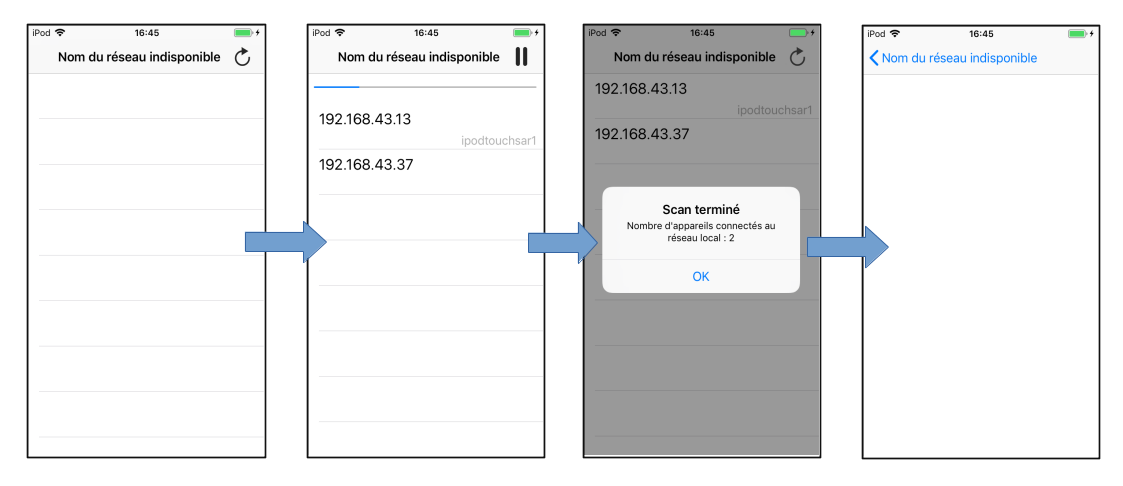
\includegraphics[scale=0.37]{iPod_file_finder.png}
		\end{center}	
	\end{frame}
	
	\begin{frame}
	\section{Prototype interface graphique}
		\begin{center}
		\frametitle{Prototype d'interface graphique Gtk+}		
		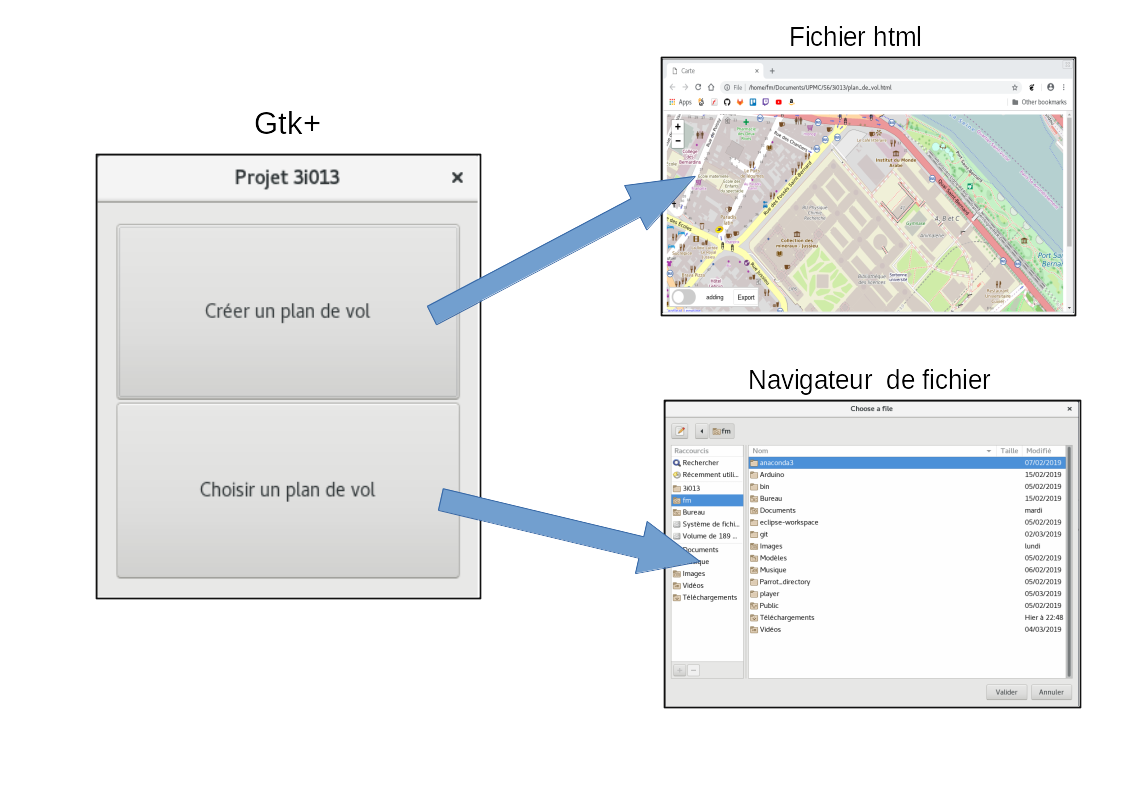
\includegraphics[scale=0.35]{schema_GUI.png}
		\end{center}
	\end{frame}
	
\end{document}
